\documentclass[UTF8,a4paper,12pt]{ctexart}

\usepackage{geometry}
\usepackage{graphicx}
\usepackage{booktabs}
\usepackage{float}
\usepackage{hyperref}
\usepackage{xcolor}
\usepackage{amsmath}
\usepackage{caption}
\usepackage{subcaption}
\usepackage{enumitem}

\geometry{left=2.5cm,right=2.5cm,top=2.5cm,bottom=2.5cm}
\hypersetup{
    colorlinks=true,
    linkcolor=blue,
    urlcolor=blue,
    citecolor=blue
}

\title{深度学习与空间智能期中作业 Task 2\\场景目标检测与视频多目标跟踪}

\begin{document}

\maketitle

\begin{abstract}
实验针对道路交通场景目标检测与多目标跟踪任务，使用 Road Vehicle Images Dataset 对 YOLO 系列单阶段目标检测模型进行微调，得到面向道路车辆场景的检测模型。实验比较了 YOLOv8n、YOLOv8s 与 YOLO11s 三种模型，其中 YOLOv8s 在本次验证集上取得最高的 mAP@0.5:0.95，因此被选为后续视频跟踪阶段的检测器。在测试阶段，实验将 YOLOv8s 与 BoT-SORT 多目标跟踪算法结合，对交通视频进行逐帧检测与目标关联，输出目标类别、置信度、Bounding Box 和 Tracking ID。进一步地，实验分析遮挡场景下目标丢失与 ID 跳变的原因，并基于检测框中心点与 Tracking ID 的连续性实现单方向越线计数。
\end{abstract}

\section{任务简介}

本任务要求完成道路场景中的目标检测与视频多目标跟踪。具体包括：
\begin{enumerate}[label=(\arabic*)]
    \item 使用 Road Vehicle Images Dataset 微调训练 YOLOv8 或同类现代单阶段目标检测模型；
    \item 准备 10--30 秒测试视频，使用训练好的模型进行视频流检测与多目标跟踪；
    \item 选取目标遮挡或密集交汇片段，展示连续 3--4 帧并分析 Tracking ID 是否稳定；
    \item 在视频画面中设置虚拟计数线，基于检测框中心点与 Tracking ID 实现越线计数。
\end{enumerate}

\section{实验数据与方法}

\subsection{训练与验证数据}

实验使用 Road Vehicle Images Dataset 作为检测模型微调数据集。该数据集包含多类道路交通目标，标注格式为 YOLO 检测格式。训练和验证阶段存在人工标注的 ground truth bounding boxes；模型输出的 bounding boxes 会与人工标注框按照类别和 IoU 阈值进行匹配，从而计算 Precision、Recall 和 mAP 等指标。数据集划分如下：

\begin{table}[H]
    \centering
    \caption{Road Vehicle Images Dataset 划分}
    \begin{tabular}{lccc}
        \toprule
        划分 & 图像数量 & 标注数量 & 用途 \\
        \midrule
        Train & 2704 & 2704 & 模型训练 \\
        Validation & 300 & 300 & 模型验证与模型选择 \\
        \bottomrule
    \end{tabular}
\end{table}

数据集共包含 21 个类别，包括 ambulance、bus、car、motorbike、pickup、truck、van 等道路车辆或交通相关目标。由于训练数据主要面向道路车辆目标，后续视频检测、跟踪与越线计数均以车辆类目标为主。

\subsection{测试视频}

测试阶段使用一段 30 秒街景交通视频进行评估。视频经过预处理后统一为 MP4 格式，并保留 30 FPS 帧率。选取的视频包含车辆通行、行人背景以及车辆交汇/遮挡场景，可用于观察多目标跟踪与 ID 稳定性问题。由于测试视频没有逐帧人工标注，视频中的检测框均为模型经过置信度阈值过滤与 NMS 后保留下来的预测框。

\subsection{检测模型}

实验采用 YOLO 系列现代单阶段检测模型作为基础模型，模型以 COCO 预训练权重初始化，并在 Road Vehicle Images Dataset 上微调至 21 个道路交通类别。主要训练并比较 YOLOv8n、YOLOv8s、YOLO11s 三种模型。


\subsection{多目标跟踪算法}

在视频阶段，实验使用训练后的检测模型逐帧输出检测框，并结合 BoT-SORT/ByteTrack 进行目标关联。Tracking ID 并非由 YOLO 检测头直接产生，而是由跟踪算法根据相邻帧检测框与历史轨迹的匹配结果分配。若当前检测框能够与已有轨迹匹配，则沿用原 ID；若匹配失败，则会初始化新轨迹并分配新的 ID。

实验主要使用 BoT-SORT 作为多目标跟踪算法，并使用 ByteTrack 作为可选对比。BoT-SORT 属于 tracking-by-detection 类型的多目标跟踪算法，依赖检测结果、运动预测和跨帧匹配来维持目标身份。对于每一帧，输出结果包括：
\begin{itemize}
    \item Bounding Box：目标位置；
    \item Class Label：目标类别；
    \item Confidence：检测置信度；
    \item Tracking ID：跨帧目标身份编号。
\end{itemize}

\section{实验设置}

\subsection{训练设置}

\begin{table}[H]
    \centering
    \caption{主要训练超参数}
    \begin{tabular}{lc}
        \toprule
        参数 & 设置 \\
        \midrule
        Framework & PyTorch + Ultralytics \\
        GPU & NVIDIA RTX 4090 \\
        Input size & 640$\times$640 \\
        Batch size & 32 \\
        Epochs & 80 \\
        Optimizer & SGD \\
        Initial learning rate & 0.01 \\
        LR schedule & Cosine decay \\
        Early stopping patience & 20 \\
        Loss function & YOLO detection loss: box loss + classification loss + DFL loss \\
        Evaluation metrics & Precision, Recall, mAP@0.5, mAP@0.5:0.95 \\
        \bottomrule
    \end{tabular}
\end{table}

训练过程中，检测模型的损失由边界框回归损失、分类损失以及 Distribution Focal Loss 组成。模型选择主要依据验证集上的 mAP@0.5:0.95，并结合 Recall 对视频跟踪连续性的影响进行判断。

\subsection{实验配置}

\begin{table}[H]
    \centering
    \caption{实验配置列表}
    \begin{tabular}{lccccc}
        \toprule
        实验名称 & 模型 & Epoch & Batch & LR & Img size \\
        \midrule
        yolov8s\_e80\_img640\_b32\_lr001 & YOLOv8s & 80 & 32 & 0.01 & 640 \\
        yolov8n\_e80\_img640\_b32\_lr001 & YOLOv8n & 80 & 32 & 0.01 & 640 \\
        yolo11s\_e80\_img640\_b32\_lr001 & YOLO11s & 80 & 32 & 0.01 & 640 \\
        \bottomrule
    \end{tabular}
\end{table}

\subsection{测试与跟踪设置}

视频测试阶段先使用 YOLOv8s 的 best.pt 作为统一检测器，再在多组 tracker 与置信度阈值设置下运行跟踪。主实验采用 BoT-SORT, conf=0.25；为分析遮挡场景中的 ID 跳变是否由单一 tracker 或置信度阈值造成，额外比较 BoT-SORT 在不同 conf 阈值下的结果，并加入 ByteTrack 作为对照。
\begin{table}[H]
    \centering
    \caption{视频跟踪设置}
    \begin{tabular}{lp{9cm}}
        \toprule
        参数 & 设置 \\
        \midrule
        Detector & YOLOv8s best.pt \\
        Tracker & BoT-SORT（主实验与阈值对比），ByteTrack（对照实验） \\
        Confidence threshold & BoT-SORT: 0.15, 0.25, 0.35；ByteTrack: 0.25 \\
        Main setting & BoT-SORT, conf=0.25 \\
        IoU threshold & 0.5 \\
        Input video length & 30 s \\
        Output & Bounding Box、类别、置信度、Tracking ID \\
        \bottomrule
    \end{tabular}
\end{table}

\section{实验结果}

\subsection{检测模型定量结果}

\begin{table}[H]
    \centering
    \caption{验证集检测结果}
    \begin{tabular}{lccccc}
        \toprule
        模型 & Best Epoch & Precision & Recall & mAP@0.5 & mAP@0.5:0.95 \\
        \midrule
        YOLOv8s & 53 & 0.5176 & 0.5765 & 0.5431 & 0.3105 \\
        YOLO11s & 61 & 0.6010 & 0.4573 & 0.5179 & 0.2927 \\
        YOLOv8n & 69 & 0.6875 & 0.3912 & 0.4456 & 0.2706 \\
        \bottomrule
    \end{tabular}
\end{table}

表中结果显示，YOLOv8s 在 mAP@0.5 和 mAP@0.5:0.95 上均为三组模型中最高，说明其在本次验证集上的检测指标相对更优。YOLO11s 的 Precision 更高但 Recall 更低，表明它输出的检测框更保守，误检相对较少，但漏检风险更高。对于视频多目标跟踪而言，漏检可能导致跟踪器无法在连续帧中匹配目标，进而造成目标丢失或 ID 跳变。因此，后续跟踪与越线计数实验采用 YOLOv8s 的 best.pt 作为检测器。

mAP@0.5 表示当预测框与人工标注框的 IoU 大于 0.5 时即视为定位正确；mAP@0.5:0.95 则在 IoU=0.50,0.55,\dots,0.95 多个阈值上计算 AP 后取平均，对定位质量的要求更高。

\subsection{训练过程可视化}

图 \ref{fig:training_curves} 展示了 YOLOv8s 训练过程中训练集与验证集的 loss 曲线，以及验证集 Precision、Recall、mAP@0.5 和 mAP@0.5:0.95 曲线。训练曲线用于观察模型是否正常收敛，以及验证集 mAP 是否在训练后期趋于稳定。

\begin{figure}[H]
    \centering
    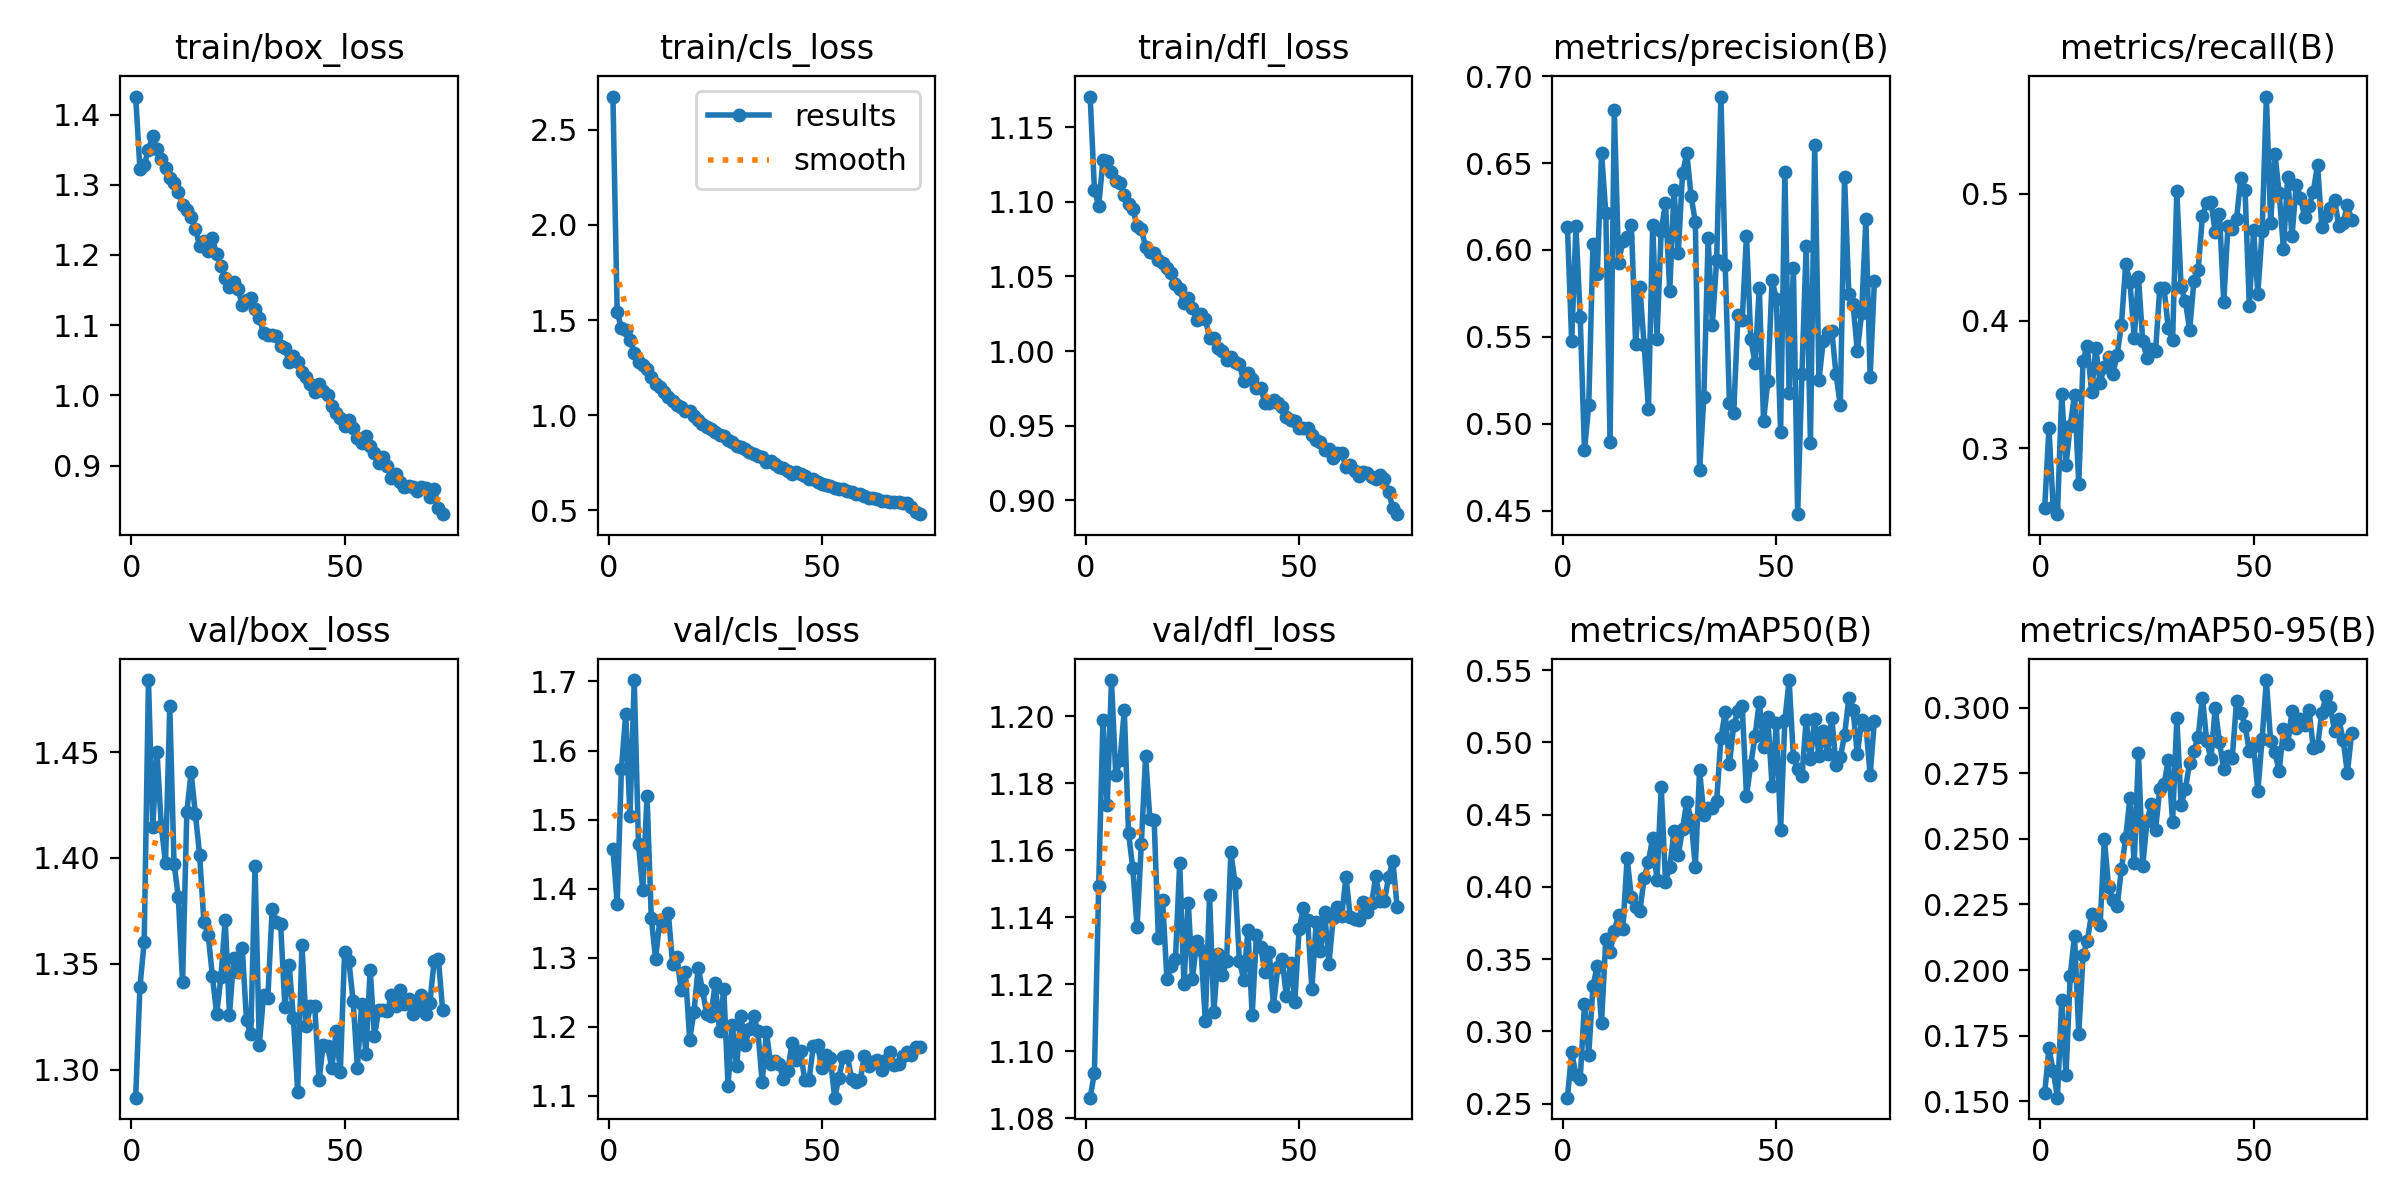
\includegraphics[width=0.92\linewidth]{figures/baseline_yolov8s_results.png}
    \caption{YOLOv8s 训练过程 loss 与 mAP 曲线}
    \label{fig:training_curves}
\end{figure}

图 \ref{fig:pr_confusion} 展示了 YOLOv8s 在验证集上的 PR 曲线和归一化混淆矩阵。PR 曲线反映了模型在不同置信度阈值下 Precision 与 Recall 的变化关系，混淆矩阵则展示了各类别之间的误检与混淆情况。

\begin{figure}[H]
    \centering
    \begin{subfigure}{0.48\linewidth}
        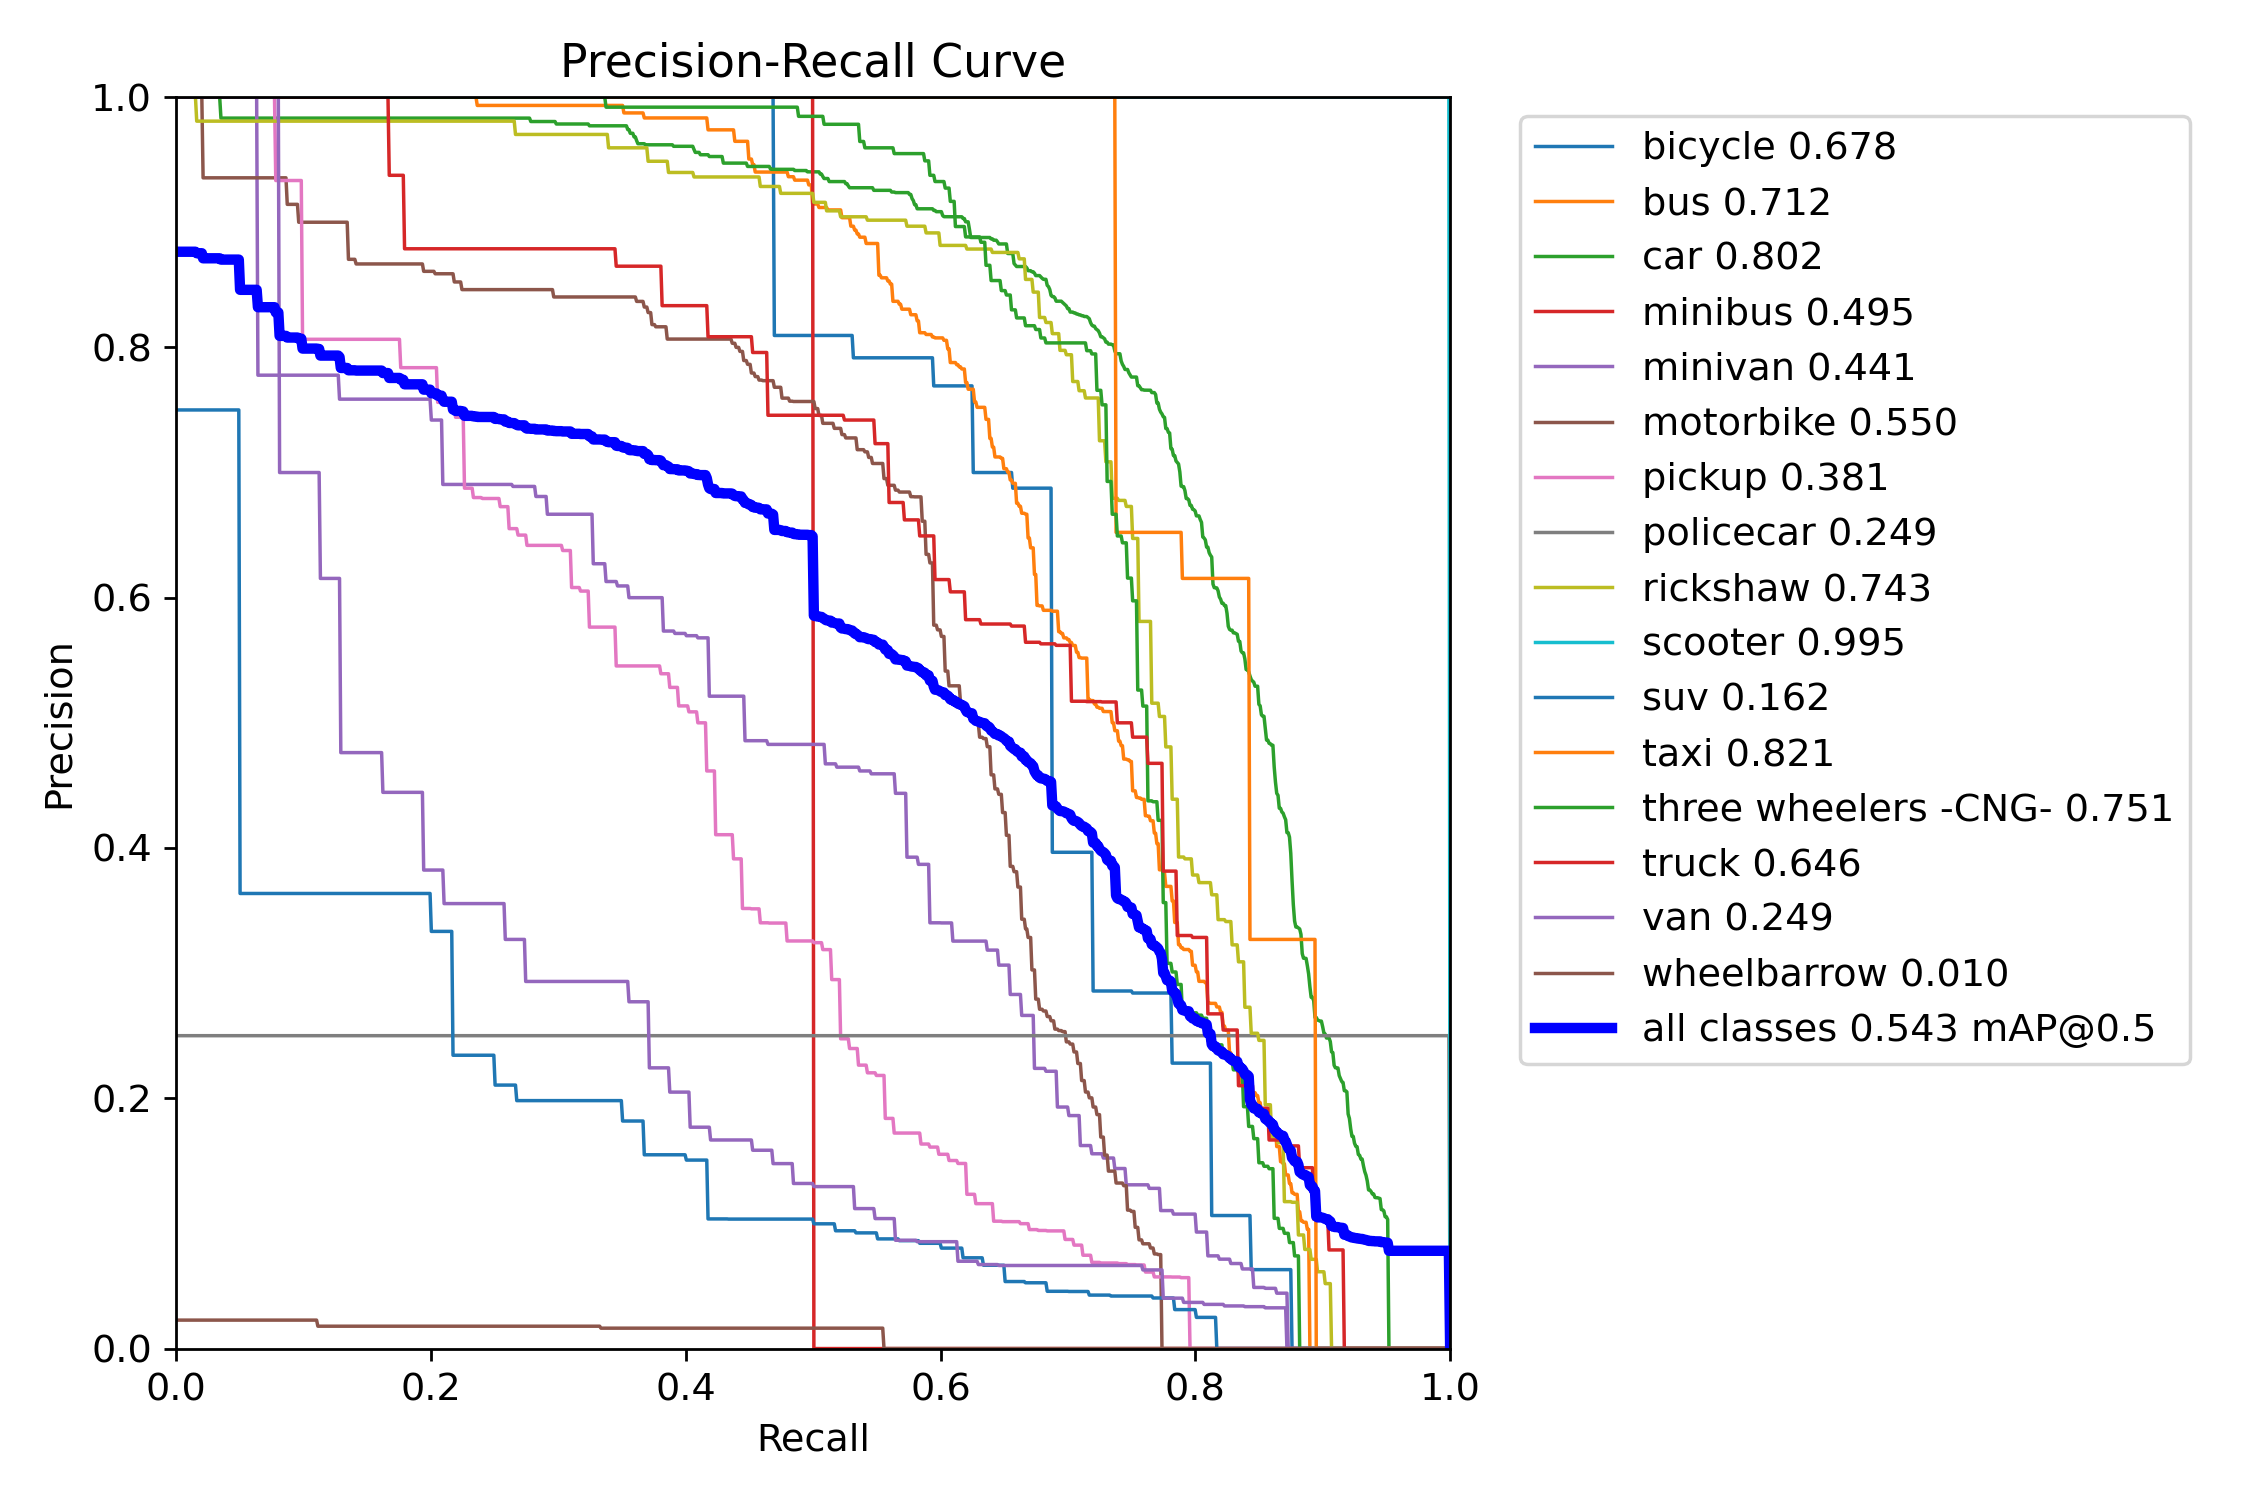
\includegraphics[width=\linewidth]{figures/baseline_yolov8s_pr_curve.png}
        \caption{PR curve}
    \end{subfigure}
    \begin{subfigure}{0.48\linewidth}
        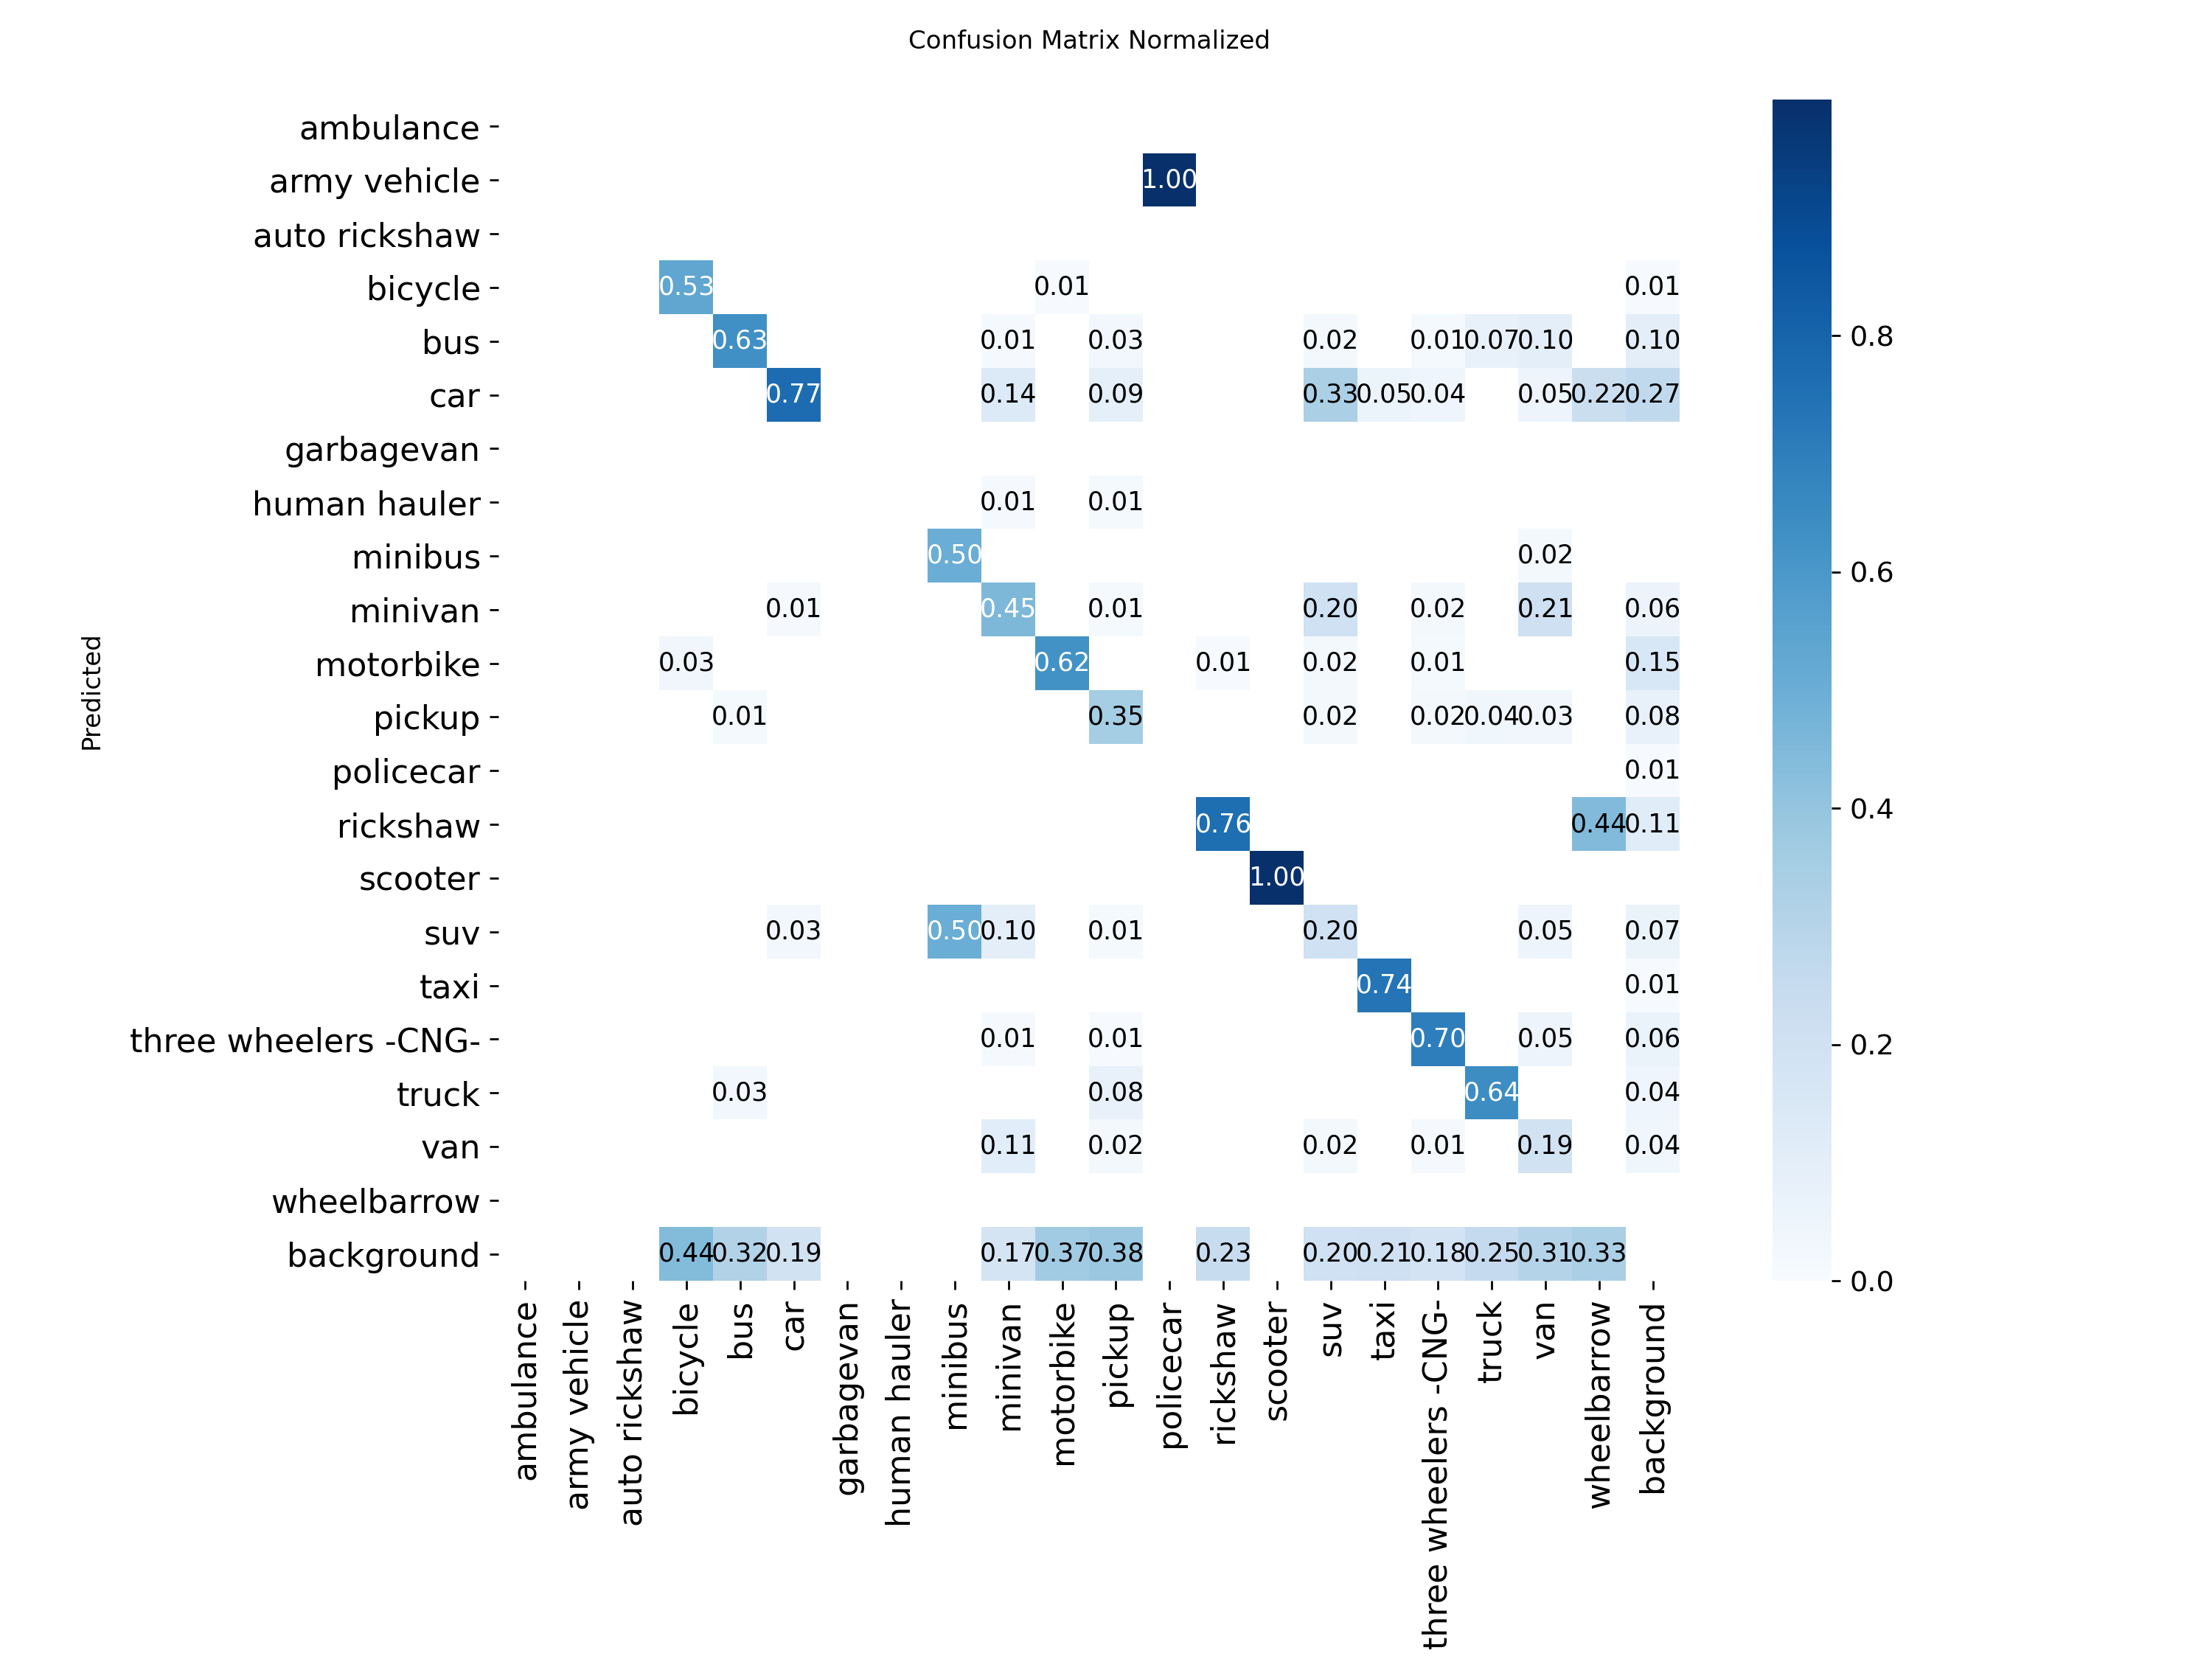
\includegraphics[width=\linewidth]{figures/baseline_yolov8s_confusion_matrix_normalized.png}
        \caption{Normalized confusion matrix}
    \end{subfigure}
    \caption{YOLOv8s 验证集 PR 曲线与归一化混淆矩阵}
    \label{fig:pr_confusion}
\end{figure}

图 \ref{fig:val_pred} 给出了验证集上的预测可视化示例。模型能够对主要车辆目标输出检测框、类别和置信度；但在小目标、遮挡目标和密集目标附近仍可能出现漏检或定位不准，这也是后续视频跟踪中目标丢失和 ID 跳变的重要来源。

\begin{figure}[H]
    \centering
    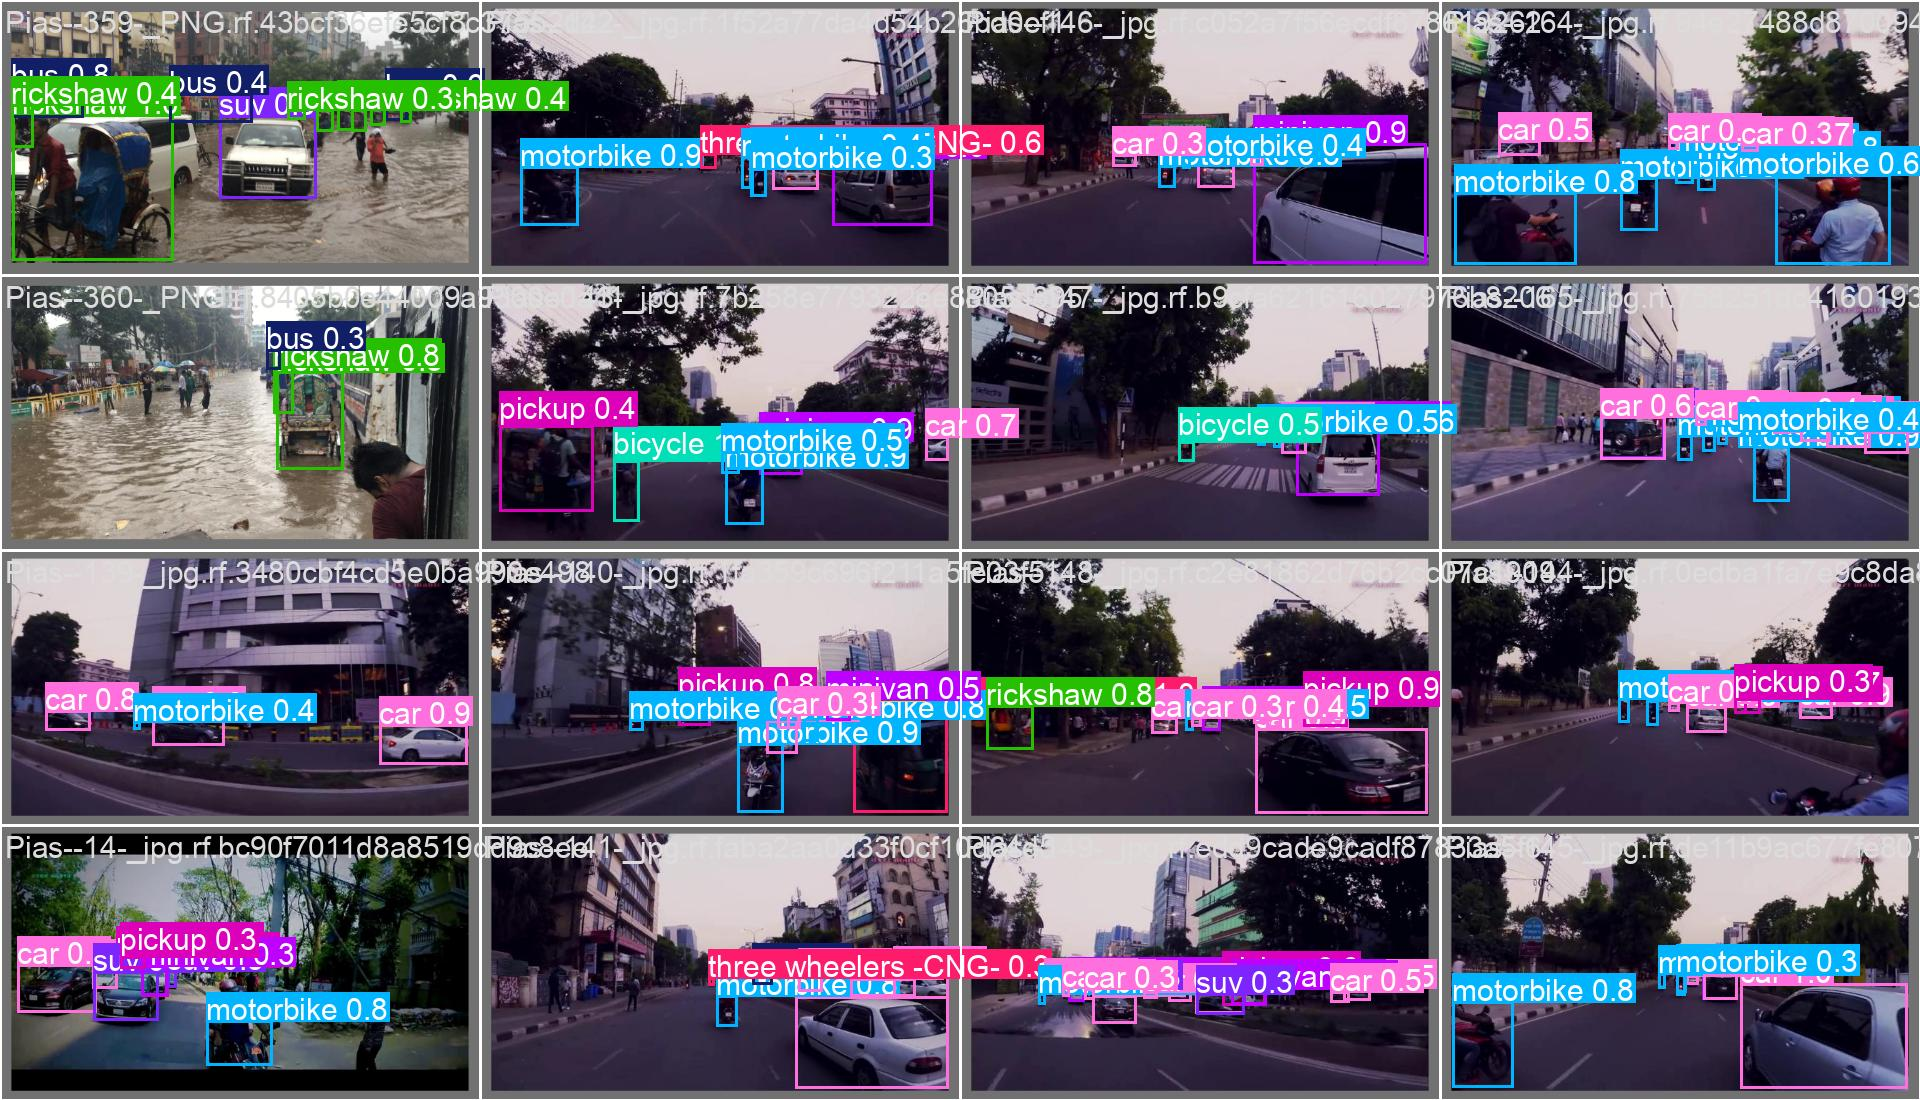
\includegraphics[width=0.9\linewidth]{figures/baseline_yolov8s_val_batch0_pred.jpg}
    \caption{YOLOv8s 验证集预测示例}
    \label{fig:val_pred}
\end{figure}

\section{遮挡与 ID 跳变分析}

实验从测试视频中选取车辆遮挡与密集交汇片段进行分析。由于测试视频为 30 FPS，严格相邻的 3--4 帧时间跨度仅约 0.1 秒，视觉变化不明显；因此从同一连续遮挡事件中选取 4 个关键帧进行可视化，以展示目标从接近遮挡、发生遮挡到重新出现的过程。图 \ref{fig:occlusion_frames} 展示了该片段的跟踪结果。本文将目标丢失定义为真实车辆仍位于画面内，但其检测框或跟踪框在若干帧中消失；将 ID 跳变定义为同一真实车辆仍被检测到，但 Tracking ID 在连续或近连续片段中发生改变。

\begin{figure}[!htbp]
    \centering
    \begin{subfigure}{0.48\linewidth}
        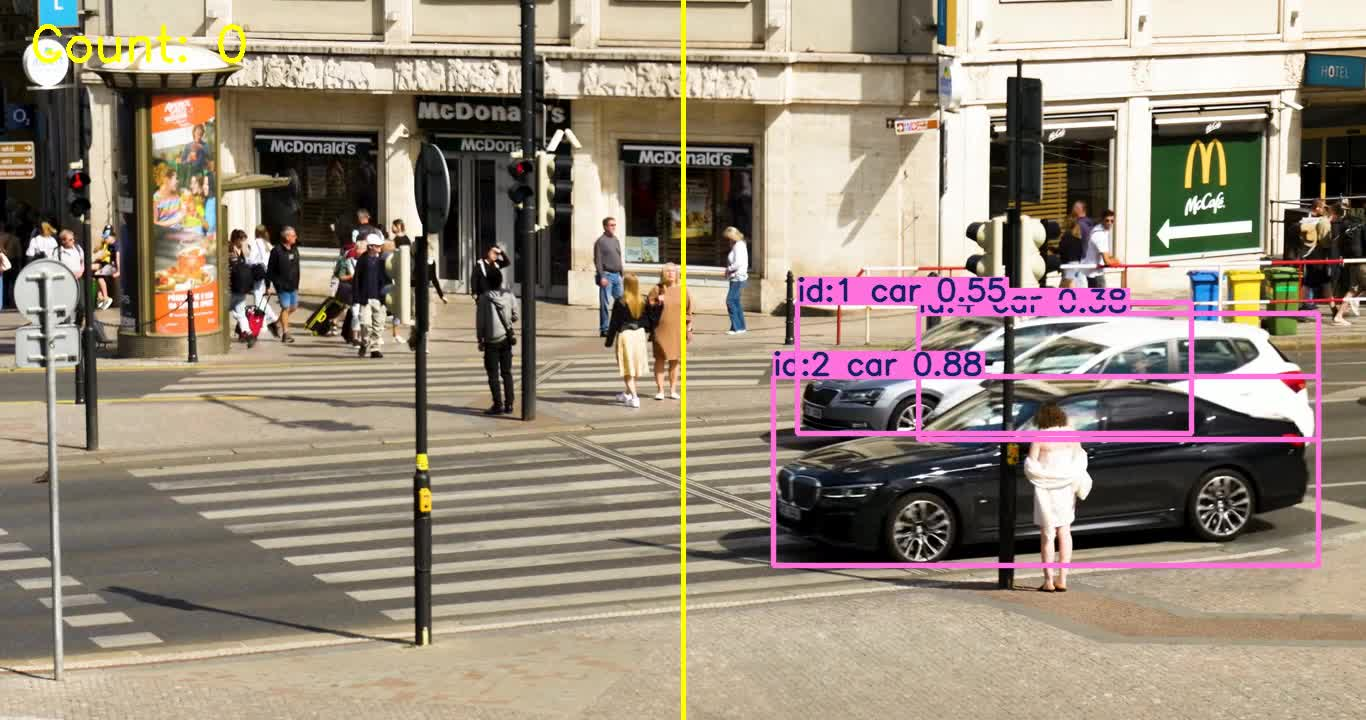
\includegraphics[width=\linewidth]{figures/test_2_botsort_conf025_occlusion_34.jpg}
        \caption{Frame 34}
    \end{subfigure}
    \hfill
    \begin{subfigure}{0.48\linewidth}
        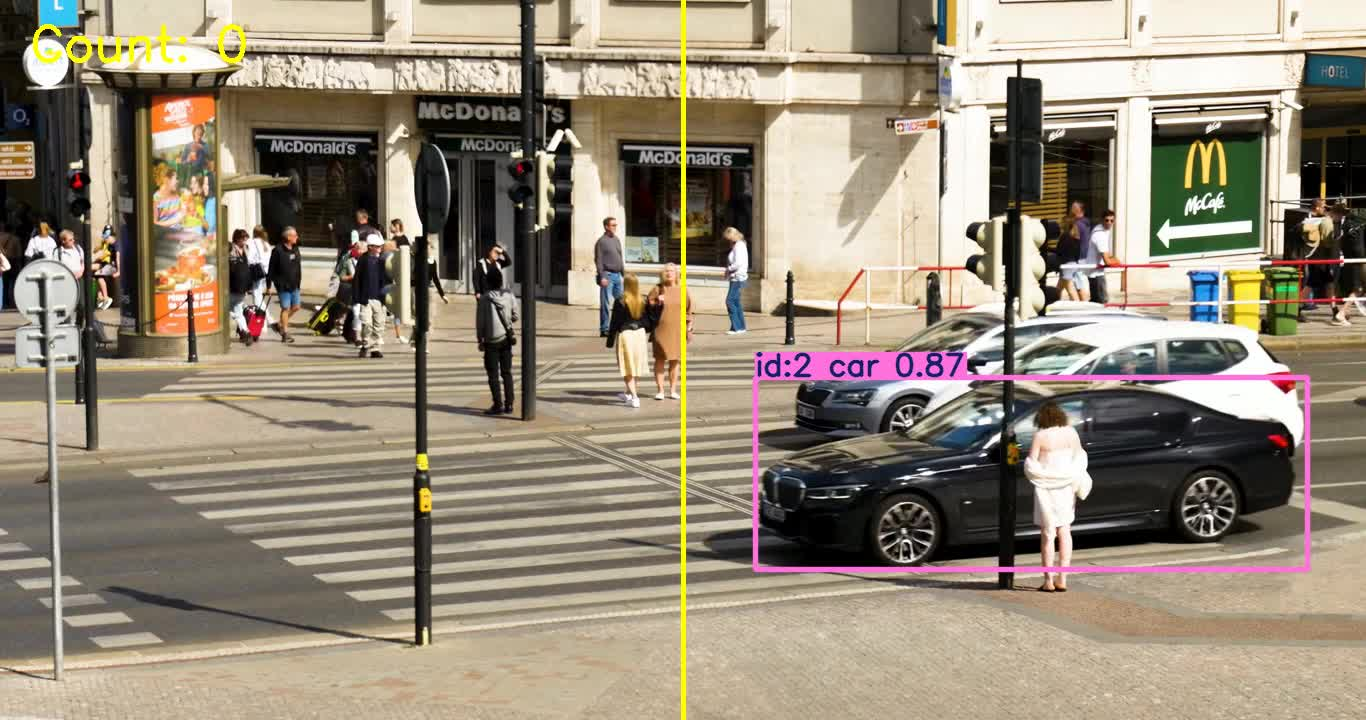
\includegraphics[width=\linewidth]{figures/test_2_botsort_conf025_occlusion_35.jpg}
        \caption{Frame 35}
    \end{subfigure}

    \vspace{0.4em}

    \begin{subfigure}{0.48\linewidth}
        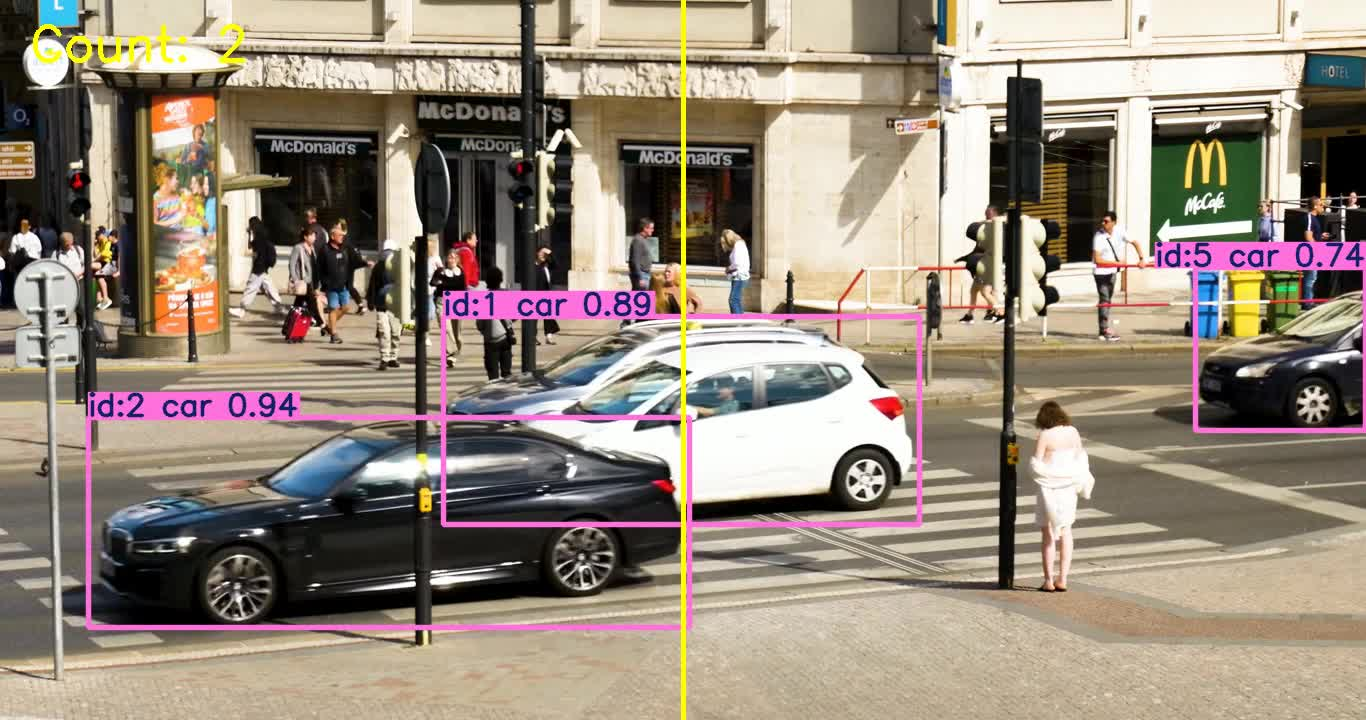
\includegraphics[width=\linewidth]{figures/test_2_botsort_conf025_occlusion_71.jpg}
        \caption{Frame 71}
    \end{subfigure}
    \hfill
    \begin{subfigure}{0.48\linewidth}
        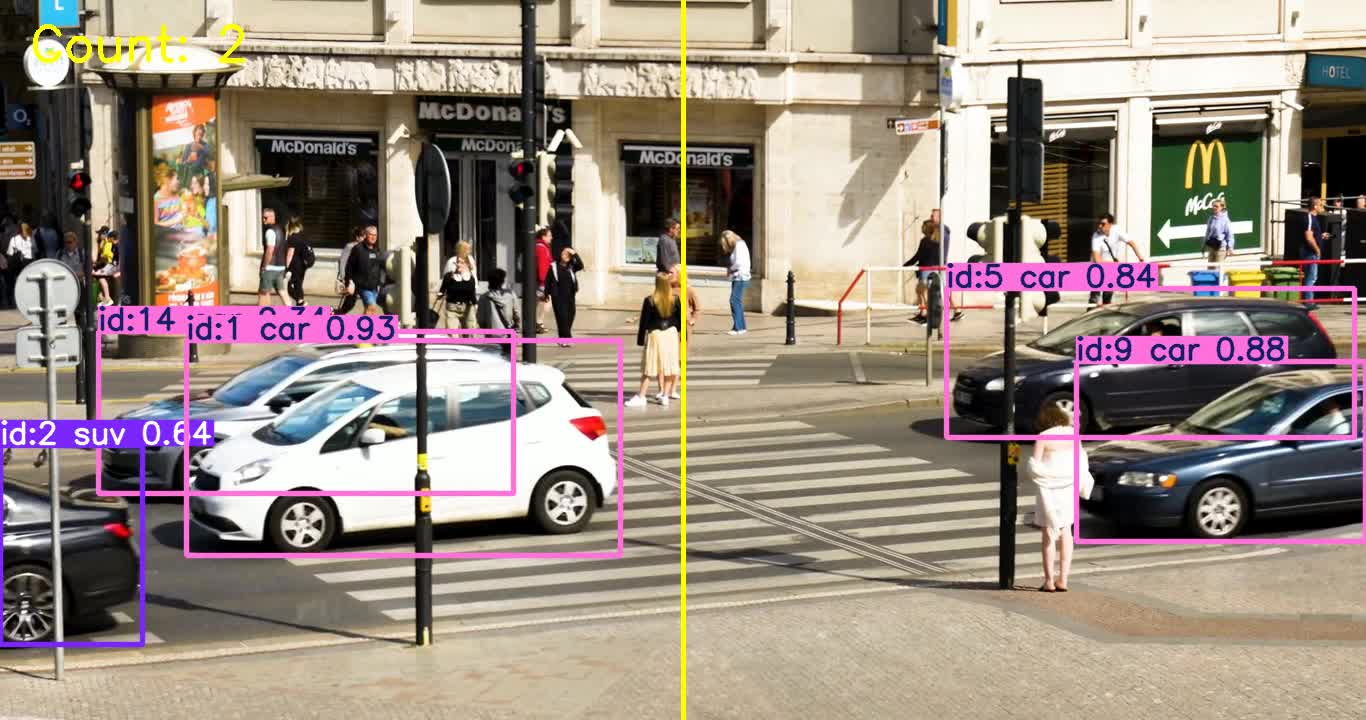
\includegraphics[width=\linewidth]{figures/test_2_botsort_conf025_occlusion_97.jpg}
        \caption{Frame 97}
    \end{subfigure}
    \caption{BoT-SORT, conf=0.25 下遮挡与 ID 跳变片段关键帧可视化}
    \label{fig:occlusion_frames}
\end{figure}

\begin{table}[H]
    \centering
    \caption{遮挡片段 Tracking ID 分析}
    \label{tab:occlusion_id_analysis}
    \begin{tabular}{lp{4cm}p{7cm}}
        \toprule
        帧 & Tracking ID & 现象 \\
        \midrule
        Frame 34 & id:4, id:1 & 两辆白车在画面右侧并行接近，检测框开始重叠，其中 id:4 位于上方车辆，id:1 位于下方车辆。 \\
        Frame 35 &  & 两车重叠进一步加剧，同时黑车遮挡白车，两辆白车 id 丢失。 \\
        Frame 71 & id:1 & 车辆通过计数线附近后黑车遮挡消失，重新检测到白车，但上方车辆为 id:1。 \\
        Frame 97 & id:1, id:14 & 白车重叠分开，重新检测到下方白车，但 id:14，因此未被计数 \\
        \bottomrule
    \end{tabular}
\end{table}

表 \ref{tab:occlusion_id_analysis} 显示，该片段的问题不是简单的框位置偏差，而是先发生目标丢失，再引发后续 ID 跳变。Frame 34 中两辆白车仍分别保持为 id:4 和 id:1；到 Frame 35 时，两辆白车进一步重叠，并受到前景黑车遮挡，两个原有 ID 均未显示，说明跟踪器在该帧没有为这两个目标保留稳定轨迹输出。遮挡解除后，Frame 71 中上方白车重新被检测到，但其 ID 变为 id:1，不再延续 Frame 34 中的 id:4；Frame 97 中下方白车重新出现为 id:14，也没有延续原先的 id:1。

目标丢失后能否重新分配回同一 ID，取决于重新出现的检测框能否与丢失前的历史轨迹重新匹配。对于 BoT-SORT 这类 tracking-by-detection 方法，匹配主要依赖检测框是否在遮挡期间仍被保留、丢失轨迹在 tracker 中保留的时间、当前检测框与历史轨迹预测位置的距离或 IoU、目标外观特征相似度，以及周围是否存在相似车辆竞争匹配。若遮挡时间较短、车辆运动方向稳定、重新出现位置接近预测位置，且周围没有相似目标，则旧轨迹更可能继续沿用原 ID。相反，当遮挡导致检测框完全消失，或者两辆白车外观相近、空间位置接近、检测框重叠严重时，tracker 难以判断重新出现的检测框应接回哪条历史轨迹，旧轨迹可能被终止，新检测框则被分配新的 Tracking ID，或被关联到另一条相近轨迹。

因此，该片段中的 ID 跳变主要由遮挡期间的目标丢失触发。Frame 35 中两辆白车的原有 ID 同时消失，使后续重关联缺少连续观测约束；Frame 71 和 Frame 97 中车辆重新出现时，id:4 未能延续到上方白车，原先的 id:1 也未能延续到下方白车。对于越线计数而言，程序依赖同一 Tracking ID 在跨线前后的连续轨迹；当下方白车在重新出现后变为 id:14 时，原轨迹被切断，因此该车辆未被计入最终计数。

为检查该失败现象是否对 tracker 或置信度阈值高度敏感，实验对比了 BoT-SORT 在不同 conf 阈值下的结果，以及 ByteTrack 在相同 conf=0.25 下的结果。表 \ref{tab:tracking_setting_comparison} 作为补充观察，用于说明这些常见设置是否能明显消除遮挡片段中的目标丢失和 ID 不连续现象。

\begin{table}[H]
    \centering
    \caption{不同 tracking 设置下遮挡片段现象对比}
    \label{tab:tracking_setting_comparison}
    \begin{tabular}{lp{1.6cm}p{4.1cm}p{4.1cm}}
        \toprule
        设置 & 程序计数 & 遮挡片段观察 & 结论 \\
        \midrule
        BoT-SORT, conf=0.15 & 36 & 与主设置相似，仍出现遮挡后的 ID 不连续 & 未明显消除该失败现象 \\
        BoT-SORT, conf=0.25 & 36 & 主实验设置，出现表 \ref{tab:occlusion_id_analysis} 所示目标丢失与 ID 跳变 & 作为baseline \\
        BoT-SORT, conf=0.35 & 35 & 现象整体相似，但程序计数略低 & 提高阈值未带来明显改善 \\
        ByteTrack, conf=0.25 & 36 & 现象整体相似，仍出现遮挡后的 ID 不连续 & 更换 tracker 未明显消除问题 \\
        \bottomrule
    \end{tabular}
\end{table}

上述结果不适合用于判断某一 tracker 或某一 conf 阈值更优，因为不同设置下的遮挡片段现象差异不明显。在该案例中，主要困难来自遮挡和车辆重叠造成的观测缺失。遮挡首先会造成检测框或跟踪框短暂消失，即目标丢失；当目标重新出现时，跟踪器还需要重新完成检测框与历史轨迹的匹配，若匹配失败则会产生 ID 跳变。越线计数依赖同一 Tracking ID 在跨线前后的连续性，因此这两类问题都会影响最终计数结果。

\section{越线计数}

\subsection{方法}

为统计视频中通过指定区域的车辆数量，实验在画面中设置一条虚拟计数线。计数视频为单向车流视频，越线计数任务定义为单方向交通流量统计。对于每个 Tracking ID，记录其检测框中心点在相邻帧中位于计数线的哪一侧。当同一 Tracking ID 的中心点沿指定方向从计数线一侧移动到另一侧，且该 ID 尚未被统计过时，计数加一。

检测框中心点计算方式为：
\begin{equation}
    c_x = \frac{x_1 + x_2}{2}, \quad c_y = \frac{y_1 + y_2}{2}
\end{equation}

若使用竖直线 $x = x_0$ 并统计从右向左的车辆，则判断目标是否跨线的条件为：
\begin{equation}
    c_x^{t-1} \geq x_0,\quad c_x^t < x_0
\end{equation}

当同一 Tracking ID 满足上述条件时，认为该目标发生一次指定方向的跨线行为。为了避免重复计数，每个 Tracking ID 只统计一次。该逻辑严格依赖 Tracking ID 的连续性，因此当目标在跨线前后发生 ID 跳变时，可能出现漏计；当同一真实目标被分配多个 ID 且多个 ID 都完成跨线时，可能出现多计。

\subsection{计数结果}

\begin{figure}[H]
    \centering
    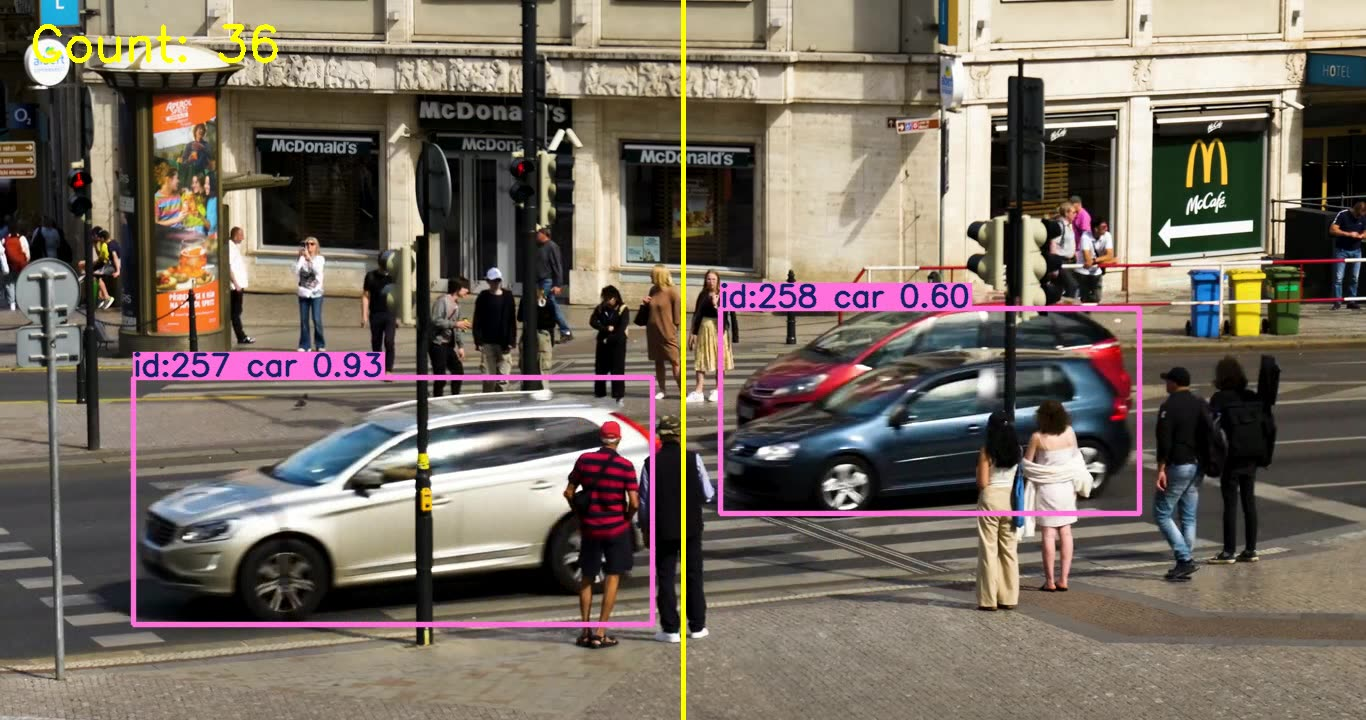
\includegraphics[width=0.9\linewidth]{figures/test_2_botsort_conf025_line_counting.jpg}
    \caption{BoT-SORT, conf=0.25 下的越线计数可视化结果}
    \label{fig:line_counting}
\end{figure}

最终测试视频中的越线计数结果为：
\begin{equation}
    \mathrm{Count} = 36
\end{equation}

实验采用人工观看视频的方式统计真实跨线车辆数，并与程序输出进行比较。若程序计数低于人工计数，可能原因包括遮挡或低置信度导致目标在跨线前后丢失，或者 ID 跳变导致程序无法确认同一目标完成了跨线；若程序计数高于人工计数，则可能由误检或同一车辆被重新分配多个 ID 后重复跨线造成。因此，越线计数不仅依赖检测模型能否识别车辆，也直接依赖 Tracking ID 的稳定性。

\begin{table}[H]
    \centering
    \caption{越线计数人工校验}
    \begin{tabular}{lcccc}
        \toprule
        视频 & 方向 & 人工计数 & 程序计数 & 误差 \\
        \midrule
        test\_2 & 右$\rightarrow$左 & 38 & 36 & -2 \\
        \bottomrule
    \end{tabular}
\end{table}

\section{结论}

实验完成了道路交通场景中的目标检测、多目标跟踪、遮挡分析与越线计数实验。通过在 Road Vehicle Images Dataset 上微调 YOLO 系列模型，得到面向道路车辆检测的模型。定量结果显示，YOLOv8s 在本次验证集上取得最高的 mAP@0.5:0.95，因此被选为后续视频跟踪检测器。在视频测试中，YOLOv8s 能够输出车辆类别、置信度和 Bounding Box，BoT-SORT 能够为多数连续目标维持 Tracking ID。遮挡分析表明，当目标被遮挡导致检测框消失或置信度降低时，跟踪器可能无法将重新出现的目标与原轨迹关联，进而发生目标丢失或 ID 跳变。越线计数实验表明，在本测试视频中，计数结果会受到检测连续性和 Tracking ID 稳定性的影响；因此，单帧检测指标、跟踪算法数据关联能力和置信度阈值设置需要结合具体场景分析。

\section*{代码与模型链接}

\begin{itemize}
    \item GitHub Repo：\url{https://github.com/QijunM0928/mllm-task2-vehicle-tracking}
    \item 模型权重下载：\url{https://pan.baidu.com/s/1ORMiWmuL8f1lhkg65jfxGw?pwd=a7e6}
\end{itemize}

\end{document}
